\section{Bringing the 3D hydrodynamical model in hydrostatic equilibrium}

Up to this point, I have specified most of the 3D hydrodynamical model's parameters, which would be simulation's starting point. However, an extremely unstable model would result from entering these values into GADGET-2, where the gas particles would quickly reach arbitrary high velocities and escape.

There are two causes for this behavior, and as a result, there are two additional phases I must complete before I can produce a smooth and stable 3D hydrodynamical model. The first is related to the softening length of the core particle, while the second is related to the initial gas particle accelerations as being calculated by GADGET-2 via gravitational forces and pressure gradients. In the next two subsection I will expand upon how I tackle these challenges. 

Furthermore, I consider an adiabatic \ac{eos}, see \cref{eq:adiabatic_eos}, with $\gamma_{ad} = 5/3$, in GADGET-2 for the gas. Hence, the simulaitons include adiabatic cooling and heating due to expansion and contraction of the gas, respectively. This decision is predicated on the fact that the simulation run time is more than two orders of magnitude shorter than the $t_{th}$ of the tertiary, see \cref{tab:tertiary_timescale_ROLF}. If $t_{th}$ was significantly shorter than the current value, an isothermal \ac{eos} may be a better choice. In order to test this assumption, I run one simulation using an isothermal \ac{eos}. As expected, the model proved extremely unstable with the envelope escaping freely since it is not affected by adiabatic cooling.

\subsection{Core particle softening length}

Since I consider the core particle to be a pure gravitational point mass with no pressure or internal energy, I need to avoid the star from collapsing on itself.
To achieve that, I use Plummer softening, $\epsilon$, to soften the core particle. Similar with GADGET-2, I adopt the conventional cubic spline of \cite{monaghan1985refined}, which drops to zero smoothly at $2.8 \epsilon$, see Eq. \eqref{eq:spline_kernel}. The density and internal energy inside the softened zone are adjusted so that pressure equilibrium is maintained while the original entropic variable $A$ is preserved, see \cref{sub:envelope_conv}. 

The motivation behind that is known as entropy sorting and it is derived by simulations of stellar collisions \citep{lombardi1995collisions,lombardi2003modelling,lombardi2006stellar,gaburov2008mixing,gaburov2010onset}, where both the entropic variable and the specific entropy are preserved in the absence of shocks and increase in their presence. To put it simply, the fluid with the highest entropy should be on top of the fluid with the lowest entropy in order to establish hydrodynamic stability. 

Defining a good $\epsilon$ has been proved a major challenge. I run a series of short convergence tests varying the number of particles $N$ and the core particle mass, $M_c$. The tests proved that the choice of the softening length, $\epsilon$, depends weakly on $N$, and strongly on $M_c$, which is related to the tertiary's mass at the moment of \ac{rlof}, see \cref{tab:core_masses_ROLF}. I demand two criteria to be fulfilled, at the same time, for selecting a good softening length:
\begin{itemize}
    \item The selected $M_c$, and hence the respective softening length, should result to a 3D density profile which agrees with MESA's 1D density profile.
    \item For a given $M_c$, and hence the respective softening length, the star should not collapse on itself at the beginning of the simulation.
\end{itemize}
The first criterion allowed me constraint my parameters' search, see \cref{fig:stellar_density_ROLF}. For the adopted $M_c$=0.255 M$_{ROLF}$, I present the parameters of the convergence tests
\begin{table}[H]
    \centering
    \begin{tabular}{| c | c | c |}
       M$_{core}$  & N & $\epsilon$/$R_{RLOF}$ \\
       \hline
       25.5\% M$_{RLOF}$ & $10^4$ & 0.1\\
       25.5\% M$_{RLOF}$ & $10^4$ & 0.15\\
       25.5\% M$_{RLOF}$ & $10^4$ & 0.2\\
       25.5\% M$_{RLOF}$ & $10^4$ & 0.25\\
       25.5\% M$_{RLOF}$ & $10^4$ & 0.3\\
       25.5\% M$_{RLOF}$ & $10^4$ & 0.4\\
       \hline
       25.5\% M$_{RLOF}$ & $50^4$ & 0.1\\
       25.5\% M$_{RLOF}$ & $50^4$ & 0.15\\
       25.5\% M$_{RLOF}$ & $50^4$ & 0.2\\
       25.5\% M$_{RLOF}$ & $50^4$ & 0.25\\
       25.5\% M$_{RLOF}$ & $50^4$ & 0.3\\
       25.5\% M$_{RLOF}$ & $50^4$ & 0.4\\
    \end{tabular}
    \caption{ Parameters of the convergence tests to adopt a softening length, $\epsilon$, for the tertiary at the beginning of \ac{rlof}.}
\label{tab:smoothing_length_exploration}
\end{table}
The tests proved that an $\epsilon \in [0.14-0.2] R_{RLOF}$ can fairly satisfy both criteria. I adopt $\epsilon = 0.16 R_{RLOF}$ which provide very good results.

At this point, it is interesting to mention that an $\epsilon \in [0.14-0.2] R_{RLOF}$ seems to satisfy the first criterion for any $0.2M_{RLOF} < M_c \leq 0.5M_{RLOF}$, given a convective envelope. After running more than 20 convergence tests varying all parameters listed in \cref{tab:smoothing_length_exploration}, I establish a rule of thumb, where $\epsilon \in [0.14-0.2] R_{RLOF}$ provides a stable hydrodynamical model given a convective envelope. This might be a good starting point for future efforts to simulate hydrodynamically stable giants with a pure gravitational point mass representing the inner high density zone.

\subsection{Relaxation}

The initial particle accelerations as determined by the \ac{sph} algorithm are not zero, despite the initial particle distribution being as smooth as feasible. This is most likely caused by a combination of factors:
\begin{enumerate}
    \item MESA and GADGET-2 adopt a different \ac{eos}. Specifically, a variable and a fixed adiabatic index $\gamma_{ad}$, respectively.
    \item Numerical artifacts of using a (scaled) regular grid in low-density region, see \cref{fig:stellar_density_ROLF}.
    \item Implications of the \ac{sph} code's implementation of gravitational softening.
    \item Treatment of particles at the surface, with anisotropic neighbour distributions.
\end{enumerate}
Neglecting these non-zero particle accelerations will produce erroneous turbulent velocities. The internal energy of the particles will subsequently grow as a result of viscous damping. Therefore, to prevent artificial heating for my model, relaxation is necessary.

Relaxation is a process that involves allowing a system to evolve over time towards its equilibrium state through the dissipation of energy. The \ac{sph} algorithm iteratively adjusts the positions $x_i$ and velocities $v_i$ of the particles based on their interactions with neighboring particles, while during the process the center-of-mass position, $R_{cm}$, and velocity $V_{cm}$ are preserved. In simple words the star oscillates towards a more hydrodynamically stable state. The internal velocities are dampened by multiplying by a factor $f$ that grows adiabatically from 0 to 1:
\begin{equation}\label{eq:adjust_positions}
    x_{i,adjusted} = x_i - R_{cm} + R_{cm,initial}
\end{equation}
\begin{equation}\label{eq:adjust_velocities}
    v_{i,adjusted} = f \times (v_i - V_{cm}) + V_{cm,initial}
\end{equation} 
Furthermore, I perform relaxation in isolation meaning that during the process the 3D hydrodynamical model is not `feeling` the potential of the inner binary. It is not easy to quantify the inherent error introduced by this assumption. The gravitational force experienced by the gas particles as a result of the binary will be proportional the mass of the binary components, and inversely proportional to their distance from them. This is a detail that may be significant in the case of simulating a triple system, where the inner binary components are relatively heavier stars and the orbital period of the outer orbit relatively shorter.

Determining the relaxation's duration is not trivial. Ideally, someone would want to perform relaxation until the model reaches a state of perfect equilibrium. On one hand, this not possible and more importantly very computationally expensive. On the other hand, taking shots in the dark is not absolutely necessary. I may start by choosing a lower and upper limit that fulfil basic physical criteria.

For the lower limit, the process should simply reduce numerical noise to an acceptable level. In simple words, at the end of the process the gas particles should be `relaxed` enough that the envelope does not escape freely. For the upper limit, the process duration should be related to the dynamical timescale of the star, see \cref{eq:dynamical_timsecale} and \cref{tab:tertiary_timescale_ROLF}. This comes from the definition of the dynamical timescale, which refers to the time needed for a star to restore dynamical equilibrium after it has been disturbed. Hence, the relaxation's duration should not be significantly longer than the dynamical timescale of the star. As a result, I choose  $t_{relax} = 10 t_{dyn}$ as an upper limit and perform the process using $n_{steps} = 100$, hence each step corresponds to $dt=0.4835$ day, see \cref{tab:tertiary_timescale_ROLF}. I present 2D maps of kinetic particle energies at $t_{relax} =[2.5, 5, 7.5, 10] t_{dyn}$.
\begin{figure}[H]
    \centering
    \begin{subfigure}[b]{0.49\textwidth}
        \centering
        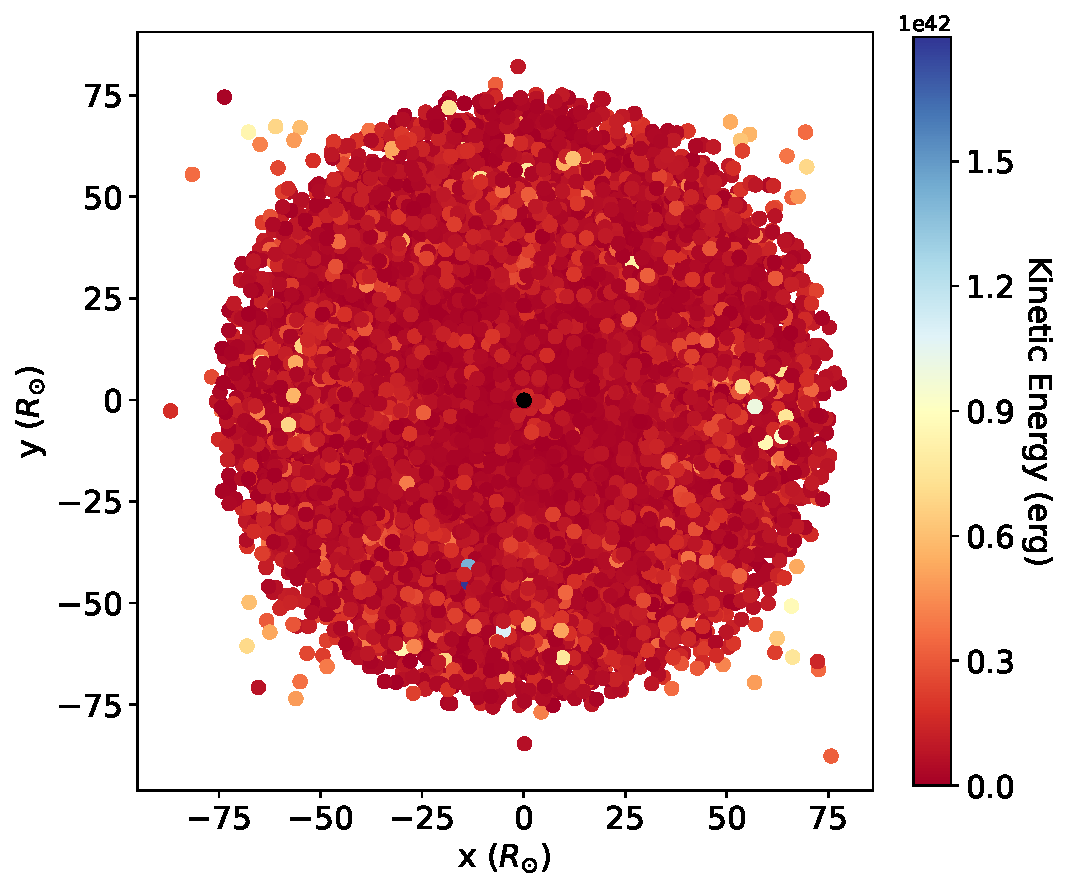
\includegraphics[width=\textwidth]{Thesis/graphs/tertiary_kin_energy_relaxed_2_5_tdyn.pdf}   
        \caption{Kinetic energies of the gas particles at  $t_{relax} = 2.5t_{dyn}$}%
    \end{subfigure}
    \hfill
    \begin{subfigure}[b]{0.49\textwidth}  
        \centering 
        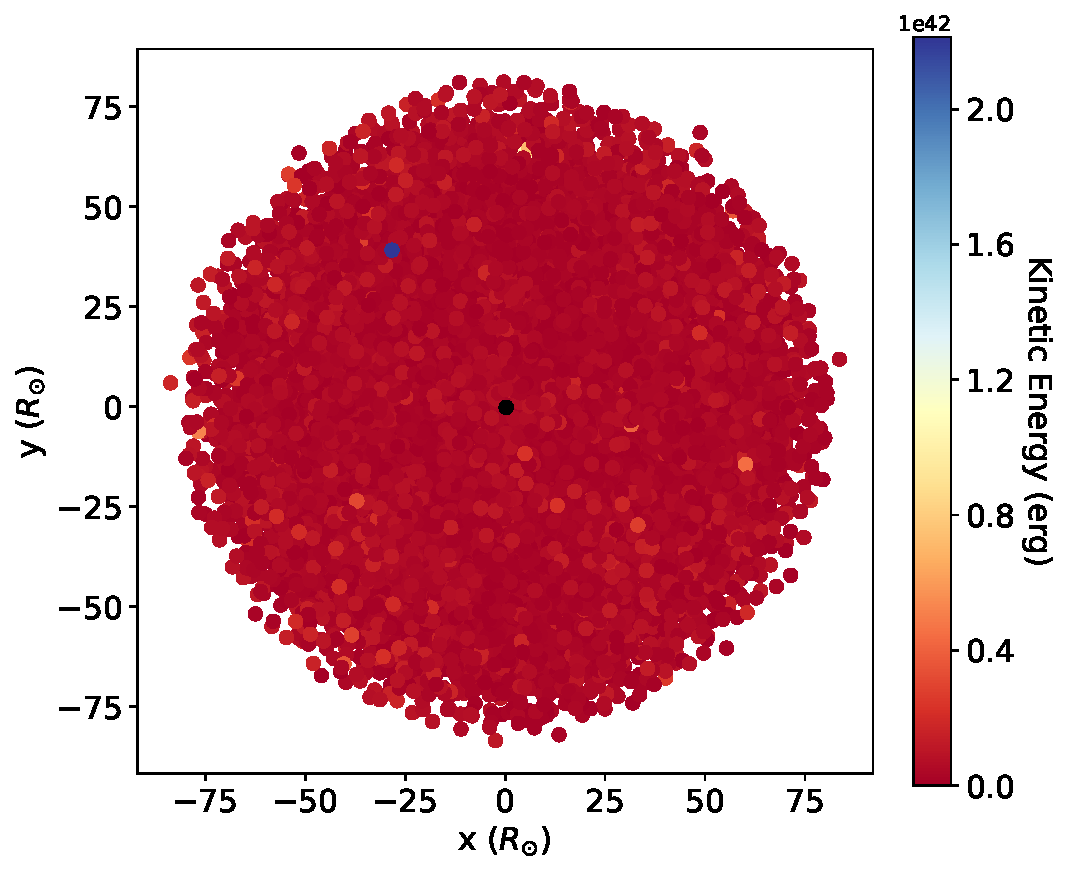
\includegraphics[width=\textwidth]{Thesis/graphs/tertiary_kin_energy_relaxed_5_tdyn.pdf}
        \caption[]%
        {{\small Kinetic energies of the gas particles at  $t_{relax} = 5t_{dyn}$}}
    \end{subfigure}
    \vskip\baselineskip
    \begin{subfigure}[b]{0.49\textwidth}  
        \centering 
        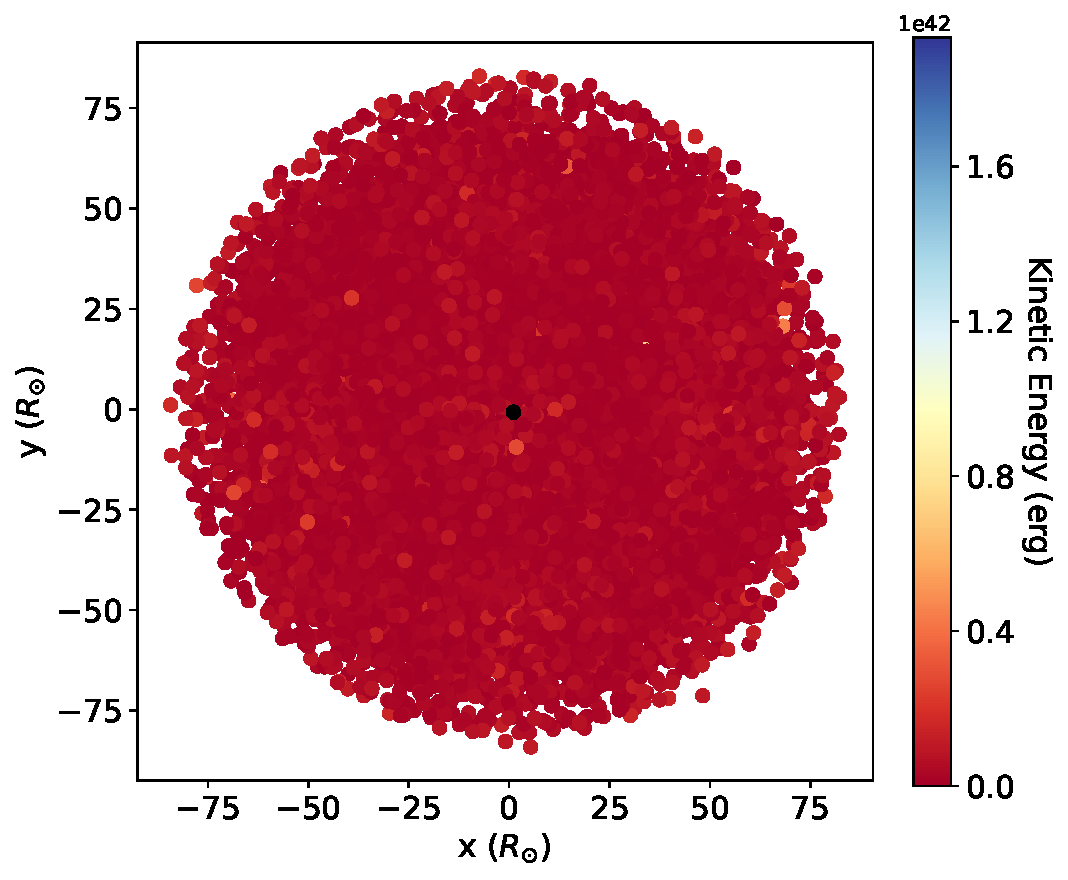
\includegraphics[width=\textwidth]{Thesis/graphs/tertiary_kin_energy_relaxed_7_5_tdyn.pdf}
        \caption[]%
        {{\small Kinetic energies of the gas particles at  $t_{relax} = 7.5t_{dyn}$}}
    \end{subfigure}
    \hfill
    \begin{subfigure}[b]{0.49\textwidth}  
        \centering 
        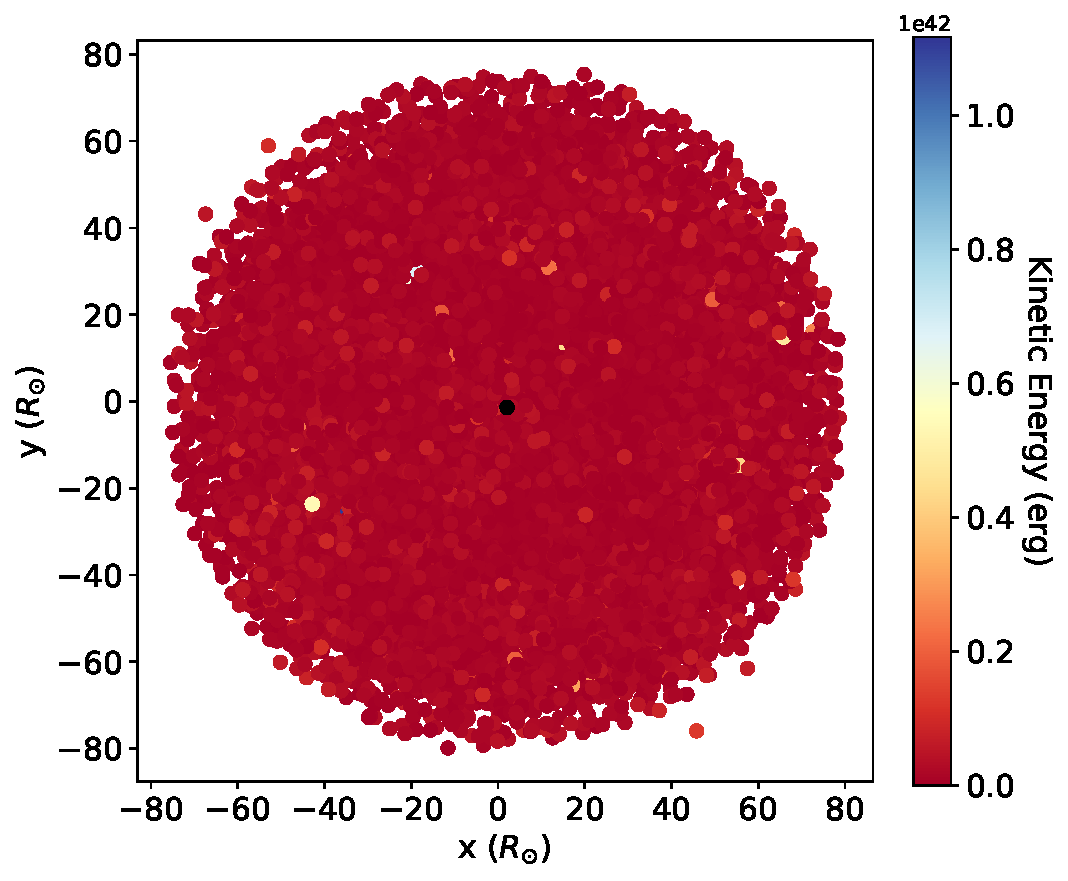
\includegraphics[width=\textwidth]{Thesis/graphs/tertiary_kin_energy_relaxed_10_tdyn.pdf}
        \caption[]%
        {{\small Kinetic energies of the gas particles at  $t_{relax} = 10t_{dyn}$}}
    \end{subfigure}
    \caption{2D maps of gas particles kinetic energies during relaxation.
    The chronological order is from left to right and from top to bottom as depicted on the respective labels. The black point corresponds to the core particle which is a pure gravitational point mass with no pressure or internal energy.}
    \label{fig:kin_energy_maps_relaxation}
\end{figure}
\cref{fig:kin_energy_maps_relaxation} shows the re-adjustment of particle positions and velocities based on \cref{eq:adjust_positions} and \cref{eq:adjust_velocities}. As the 3D hydrodynamical model becomes more spherically symmetric and the particles' kinetic energy decreases, it gradually moves towards a more hydrodynamically stable state. The latter is more apparent in \cref{fig:total_kin_energy_relaxation}, where
I present the total kinetic energy of the gas particles at $t_{relax} =[2.5, 5, 7.5, 10] t_{dyn}$.
\begin{figure}[H]
    \centering
    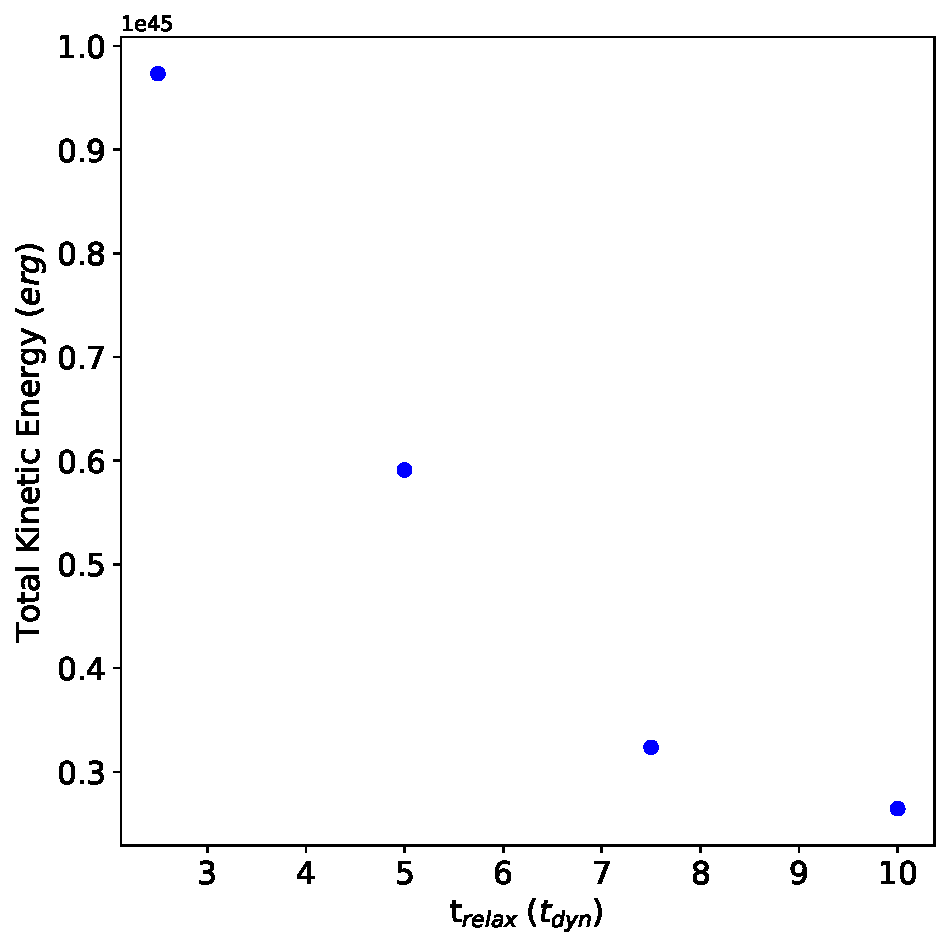
\includegraphics[width=0.9\textwidth]{Thesis/graphs/total_kientic_energy_during_relaxation.pdf}
    \caption{Evolution of the total kinetic energy of gas particles during relaxation. The blue points correspond to $t_{relax} =[2.5, 5, 7.5, 10] t_{dyn}$, respectively.}
    \label{fig:total_kin_energy_relaxation}
\end{figure}















